As we discussed in the previous section, our motivation is to use Theorem \ref*{thm_positive_rank} to predict points of infinite order for families of elliptic curves. However, in this section we prove that in several cases the theorem will never make such a prediction. In other words, in such cases, the product 
$$\frac{\prod_i C_{E/F_i}}{\prod_j C_{E/F_j'}}$$ 
is always a norm for every subfield $\QQ(\sqrt{D})\subseteq\QQ(\rho)$. Before we give the precise statements, we give a proof of some important results that will be used throughout. The first one discussed the quadratic subfields of certain cyclotomic extensions.

\begin{lemma}\label{lem_subfields}
    Let $p$ be a rational prime, $n$ a positive integer and let $p^*=(-1)^{(p-1)/2}p$. Then the following holds.

    \begin{table}[!ht]
        \centering
        \begin{tabular}{|l|l|l|}
        \hline
        Cyclotomic field                     & Conditions & Quadratic subfields                   \\ \hline
        $\QQ(\zeta_{p^n})$                   & $p$ odd, any $n$    & $\QQ(\sqrt{p^*})$            \\ \hline
        %\multirow{3}{*}{$\QQ(\zeta_{2^m})$}  & $m=1$      & none                                  \\ \cline{2-3} 
        %                                     & $m=2$      & $\QQ(i)$                              \\ \cline{2-3} 
        %                                     & $m\geq3$   & $\QQ(i),\QQ(\sqrt{2}),\QQ(\sqrt{-2})$ \\ \hline
        %\multirow{2}{*}{$\QQ(\zeta_{2^mp^n})$}  & $m=1$, $p$ odd, any $n$      & $\QQ(\sqrt{p^*})$     \\ \cline{2-3} 
        %                                     & $m=2$, $p$ odd, any $n$      & $\QQ(i),\QQ(\sqrt{p}),\QQ(\sqrt{-p})$                              \\ 
        %                                     \hline
        \end{tabular}
        \end{table}

\end{lemma}

\begin{proof}
    Firstly, we remark that the discrimant of the field $\QQ(\sqrt{D})$, with $D$ squarefree is
    \begin{equation}
        \Delta(\QQ(\sqrt{D}))=
        \begin{cases}
            D \ \quad\text{  if } D\equiv1\pmod{4},\\
            4D \quad\text{ if } D\equiv2,3\pmod{4}.
        \end{cases}
    \end{equation}
    In addition, we also recall that $\QQ(\zeta_N)/\QQ$ is a Galois extension with $\Gal(\QQ(\zeta_N)/\QQ)=(\ZZ/N\ZZ)^*$ and that a rational prime $q$ ramifies in $\QQ(\zeta_N)/\QQ$ if and only if $q\mid N$. The result follows by combining these two properties with the Galois correspondence, as we show now.

    If $p$ is odd, then $\Gal(\QQ(\zeta_{p^n})/\QQ)=(\ZZ/p^n\ZZ)^*=C_{p^{n-1}(p-1)}$ is a cyclic group of even order, and therefore $\QQ(\zeta_{p^n})$ has one unique quadratic subfield, which can only ramifiy at $p$. If $p\equiv1\pmod{4}$, then the only such field is $\QQ(\sqrt{p})$ and if $p\equiv3\pmod{4}$ the only such field is $\QQ(\sqrt{-p})$. This proves the first row. 

    Since $\QQ(\zeta_2)=\QQ$ and $\QQ(\zeta_4)=\QQ(i)$, the second and third row are immediate. For $m\geq3$, $\Gal(\QQ(\zeta_{2^m})/\QQ)=(\ZZ/2^m\ZZ)^*=C_2\times C_2^{m-2}$ and therefore $\QQ(\zeta_{2^m})$ has three quadratic subfields that can only ramify at $2$. Again, it is easy to check that the only such fields are $\QQ(i)$, $\QQ(\sqrt{2})$ and $\QQ(\sqrt{-2})$, as desired. Alternatively, one can also show that $\zeta_8=(1+i)/\sqrt{2}$, which also implies the result. This proves the third row.

    The remaining rows are essentially a combination of the results we have already shown. We note that $\Gal(\QQ(\zeta_{2p^n})/\QQ)=(\ZZ/2p^n\ZZ)^*$ is cyclic while $$\Gal(\QQ(\zeta_{2^mp^n})/\QQ)=(\ZZ/2^mp^n\ZZ)^*=(\ZZ/2^m)^*\times(\ZZ/p^n\ZZ)^*=C_2\times C_{2^{m-2}}\times C_{p^{n-1}(p-1)}.$$
    Hence, $\QQ(\zeta_{2^mp^n})$ has one unique quadratic subfield if $m=1$ which must be $\QQ(\sqrt{p^*})$, three quadratic subfields if $m=2$ which are $\QQ(i),\QQ(\sqrt{p}),\QQ(\sqrt{-p})$ and seven quadratic fields if $m=3$. In the latter case, we know that $i,\sqrt{p^*},\sqrt{2}\in\QQ(\zeta_{2^mp^n})$ and therefore the seven fields must be the ones listed in the table.

\end{proof}

The second result gives a necessary condition on primes ramifying in finite extensions. The result is naturally phrased in terms of local fields.

\begin{prop}\label{prop_totally_ramified}
    Let $F/\QQ_p$ be a finite extension with residue field $\kappa$. Then there exists a tame, totally ramified cyclic extension $F_n$ of degree $n$ over $F$ if and only if $n\mid|\kappa^*|$.
\end{prop}

\begin{proof}
    Assume first that $n\mid|\kappa^*|$. Let $\pi$ be a normalizer of $F$ and consider $F_n=F(\pi^{1/n})$. We claim that $F_n$ satisfies the desired properties. Since $n\mid|\kappa^*|$, $\kappa$ contains all $n$-th roots of unity and therefore the polynomial $x^n-1$ factors into linear terms in $\kappa[x]$. The divisibility condition above implies $\Char\kappa\nmid n$ and hence by Hensel's Lemma $x^n-1$ also factors into linear terms in $F[x]$. In other words, $\QQ_p(\zeta_n)\subseteq F$ and therefore $F_n$ is the splitting field of the polynomial $x^n-\pi$. This shows that $F_n/F$ is a tame, toally ramified Galois extension, and the map 
    \begin{align*}
        \psi: \Gal(F_n/F)&\longrightarrow \mu_n\cong C_n\\
        \sigma &\longmapsto \frac{\sigma(\pi^{1/n})}{\pi^{1/n}}
    \end{align*}
    is an isomorphism of groups, which proves that the extension is cyclic of degree $n$.

    Conversely, suppose that $F_n/F$ is a tame, totally ramified cyclic extension of degree $n$. An important result shows that there is some uniformizer $\pi$ of $F$ such that $F_n=F(\pi^{1/n})$. The polynomial $x^n-\pi$ is Einstein over $F$, and therefore irreducible over $F$. Since $F_n/F$ is assumed to be Galois, all roots of $x^n-\pi$ lie in $F_n$. In particular, $\QQ(\zeta_n)\subseteq F_n$. Since $\Char\kappa\nmid n$, it follows that $\kappa$ also contains all $n$-th roots of unity, proving that $n\nmid|\kappa^*|$ as desired. 
\end{proof}

\subsection{Cyclic Extensions}
In this subsection we prove the following. 
\begin{thm}\label{thm_consistent_cyclic}
    Let $E/\QQ$ be a semistable elliptic curve and let $F$ be a finite cyclic Galois extension of $\QQ$, so that $\Gal(F/\QQ)=C_d$ for some $d\geq 2$. Let $\chi$ be a faithful character of $C_d$ (so that $\QQ(\chi)=\QQ(\zeta_d)$), and let $F_i,F'_j\subseteq F$ be such that
    $$\bigoplus_{\fg\in\Gal(\QQ(\zeta_d)/\QQ)}\chi^{\fg}=\bigoplus_i\Ind_{F_i/\QQ}\mathds{1}\ominus\bigoplus_j\Ind_{F'_j/\QQ}\mathds{1}.$$
    Then for any $\QQ(\sqrt{D})\subseteq\QQ(\zeta_d)$,
    $$\frac{\prod_i C_{E/F_i}}{\prod_j C_{E/F_j'}}$$
    is a norm of $\QQ(\sqrt{D})$. Moreover, the contribution is always the square of rational number unless $d=2^n, p^n,2p^n$ for some odd prime $p$.
\end{thm}

The first step in proving Theorem \ref{thm_consistent_cyclic} is to show that the fields $F_i, F'_j$ exist, and to give a precise description. Recall that for each $k\mid d$ the cyclic group $C_d$ has one unique subgroup of order $k$, which is of course also cyclic. Therefore, for each $k\mid d$, there is one unique subfield $L_k$ of $F$ of degree $k$ over $\QQ$ which is also cyclic. Under the Galois correspondence, this field corresponds to the subgroup $H_k=\Gal(F/L_k)=C_{d/k}$.

To give the required description, we recall that the Möbius function $\mu$ is the function supported on the square-free integers, and $\mu(n)=(-1)^s$ whenever $n$ is square free and $s$ is the number of prime factors of $n$.

\begin{lemma}\label{lem_cyclic_decomp}
    Let $E/\QQ$, $F$ and $\chi$ be as in Theorem \ref{thm_consistent_cyclic}. Writing characters of $C_d$ additively, we have that
    \begin{equation}\label{eqn_cyclic_relation}
        \fN_{\QQ(\chi)/\QQ}(\chi)=\sum_{\fg\in\Gal(\QQ(\zeta_d)/\QQ)}\chi^{\fg}=\sum_{k\mid d}\mu(d/k)\Ind_{L_k/\QQ}\mathds{1}.
    \end{equation}
    Furthermore, such an expression is unique.
\end{lemma}

\textbf{Add reference here from the exact result in the Rep Theory section.}

\begin{rem}\label{rem_radical}
    This lemma has an important consequence. Given an integer $d\geq2$, let $\rad(d)=\prod_{p\mid d}p$ be the radical of $d$, and let $K=L_{d/\rad(d)}$ be the unique subfield of $F$ such that $[F:K]=\rad(d)$. For $k\mid d$, $\mu(d/k)\neq 0$ precisely when $[K:\QQ]=\frac{d}{\rad(d)}\mid k$ and therefore the fields appearing in the right hand side of \eqref{eqn_cyclic_relation} are the fields $L_k$ satisfying $K\subseteq L_k\subseteq F$. 
\end{rem}

Following this observation, we will compute the product of the local factors locally for each finite place $\pp$ of $K$ and the places above it in the other fields $L_k\supseteq K$. To that objective, the following notation will be useful.

\begin{notation}\label{not_local_contr}
    Let $E/\QQ$, $F$ and $\chi$ be as in Theorem \ref{thm_consistent_cyclic}, and let $L_k$ and $K$ be as in Remark \ref{rem_radical}. For a finite place $\pp$ of $K$, we write
    $$\contr_\chi(\pp)=\prod_{\frac{d}{\rad(d)}\mid k\mid d}C_{\fP\mid\pp}(E/L_k)^{\mu(d/k)}=\prod_{k\mid d}C_{\fP\mid\pp}(E/L_k)^{\mu(d/k)}$$ 
    where the terms in the product are defined as in Notation \ref{not_contr}. 
\end{notation}

An immediate consequence of the above definition is the fact that 
\begin{equation}\label{eqn_local_contr}
    \prod_{k\mid d}(C_{E/L_k})^{\mu(d/k)}=\prod_\pp\contr_\chi(\pp),
\end{equation}

and therefore we can calculate the product of local terms \textbf{locally}, one prime $\pp$ at a time.

We divide the proof of Theorem \ref{thm_consistent_cyclic} into two cases: odd and even cyclic extensions. The main idea in both cases is to simplify the general case into smaller cases where we can directly compute $\contr_\chi(\pp)$ for each finite place $\pp$ of $K$. 
%An important step of the proof is to identify all quadratic subfields of certain cyclotomic extensions of $\QQ$. The following lemma gathers everything we require.

\subsection*{Odd Cyclic Extensions} \label{case_Cp}

For the first case, we assume that $d$ is odd. Following the observation in Remark \ref{rem_radical}, we need to calculate $\contr_\chi(\pp)$ for each finite place $\pp$ of $K$. To that objective, we first calculate them for ``small'' cases and then we use them for the general case. The following lemmas build on this idea.

\begin{lemma}\label{lem_Cp}
    Let $q$ be an odd rational prime, $F/K$ a Galois extension of number fields such that $\Gal(F/K)=C_q$ and $E/\QQ$ an elliptic curve with semistable reduction at $2$ and $3$. Then 
    $$\frac{C_{E/F}}{C_{E/K}}$$
    is a norm from $\QQ(\sqrt{q^*})$.
\end{lemma}

\begin{proof}
    Fix some prime $\pp$ in $K$ and note that since the extension $L/K$ is cyclic, the splitting behaviour of $\pp$ in $L$ is determined by the ramification index $e_\pp$ and the residual degree $f_\pp$. Since $\contr_\chi(\pp)=1$ if $E$ has good reduction at $\pp$, we assume that $E$ bad reduction at $\pp$. If $\pp$ has multiplicative reduction, then $D_{\fP\mid\pp}(F/K)=1$ and the following table records the contribution of the Tamagawa numbers of $\pp$ depending on $e_\pp$ and $f_\pp$, and the entries for split and non-split multiplicative reduction of type $\mathrm{I}_n$ are separated by a ``;''. To complete these calculations, we use repeatedly Proposition \ref{prop_semi_red} and Lemmas \ref{lem_mult_tam} and \ref{lem_add_tam}. We also use Notation \ref{not_n}.

    \begin{table}[!ht]
        \centering
        \begin{tabular}{|l|l|l|l|l|}
        \hline
        $e_\pp$ & $f_\pp$  & $T_{\fP\mid \pp}(E/K)$ & $T_{\fP\mid \pp}(E/F)$  & $\contr_\chi(\pp)$ \\ \hline
        $1$ & $1$ & $n;\tilde{n}$ & $n^q;\tilde{n}^q$ & $\square$ \\ \hline
        $q$ & $1$ & $n;\tilde{n}$ & $qn;\tilde{n}$ & $q\square;\square$ \\ \hline
        $1$ & $q$ & $n;\tilde{n}$ & $n;\tilde{n}$ & $\square$ \\ \hline
        \end{tabular}
    \end{table}

    Since $q$ is indeed a norm from $\QQ(\sqrt{q^*})$ by Lemma \ref{p-norm}, it follows that $\contr_\chi(\pp)$ is a norm from $\QQ(\sqrt{q^*})$ as well.

    Now assume $\pp$ has additive reduction, and let $p\ZZ=\pp\cap\QQ$. By assumption, $p\neq2,3$. Firstly, we note that $D_{\fP\mid\pp}(E/F)=1$ unless $\pp$ ramifies in $F/K$, and in that case it is a power of $N_{K/\QQ}(\pp)=p^s$. If $s$ is even, we are immediately done, so assume instead that $s$ is odd. If $L_\fP/K_\pp$ is wildly ramified, then $p=q$ is a norm from $\QQ(\sqrt{q^*})$. If $L_\fP/K_\pp$ is tamely ramified, then by Proposition \ref{prop_totally_ramified}, it follows that $q\mid p^s-1$ and therefore 
    \begin{equation}
        \left(\frac{q^*}{p}\right)=\left(\frac{p}{q}\right)=\left(\frac{p^s}{q}\right)=1
    \end{equation}
    Therefore, $p$ splits in $\QQ(\sqrt{q^*})$ and by Lemma \textbf{insert relevant thm here}, it follows that $p$ is a norm from $\QQ(\sqrt{q^*})$. 
    Finally, we need to consider the Tamagawa numbers. Note that since $q$ is odd, if $\fP$ is any prime in $F$ above $\pp$, then $\sqrt{D}\in K_\pp$ if and only if $\sqrt{D}\in L_\fP$ for any $D\in\QQ$. Moreover, if $q\neq 3$, then $\gcd(e_{\fP\mid\pp},12)=1$ and by Lemma \ref{lem_add_tam}, $c_\pp(E/K)=c_\fP(E/F)$. Since the number of primes $\fP$ in $L$ above $\fp$ is odd, we get a square in this case. If $q=3$ and $\pp$ is unramified in $L/K$, then $e_{\fP\mid\pp}=1$ and the same reasoning shows that we get a square in this case. 

    So now assume that $q=3$ and that $L\fP/K_\pp$ is ramified. Let $n=\nu_\pp(\Delta_{E,\pp}^{\min})$ be the valuation of the minimal discriminant of $E$ at $\pp$. By Lemma \ref{lem_add_tam}, we can obtain factors of $2$ and $3$. Since $3$ is a norm from $\QQ(\sqrt{-3})$, we only need to take care of the factors of $2$, which can only arise if $F_\fP/K_\pp$ is ramified, $\gcd(n,10)=2$ and $\sqrt{\Delta}\not\in K_\pp$. However, we claim that this cannot happen, implying that the contribution must be a norm from $\QQ(\sqrt{-3})$. This is a non-trivial proof, so we prove it as a separate lemma, from which this result follows. 
\end{proof}

\begin{lemma}\label{lem_nottwo}
    Let $p\geq 5$ be a rational prime and $L_\fP/K_\fp/\QQ_p$ be finite extensions with $L_\fP/K_\fp$ Galois, ramified and $\Gal(L_\fP/K_\fp)=C_3$. Let $$E/\QQ_p:y^2=x^3+Ax+B$$ be a minimal Weierstrass equation at $\pp$ with potentially good reduction. Let $x=\nu_\pp(\Delta)$ be the valuation of the minimal discriminant. If $\gcd(n,12)=2$, then $\sqrt{\Delta}\in K_\pp$.
\end{lemma}

\begin{proof}
    The condition that $E$ has additive reduction is equivalent to $A,B\in\pp$, and the condition on ramification implies that $3\mid N(\pp)-1$ by Proposition \ref{prop_totally_ramified}. In addition, by Lemma \ref{lem_Dterms}(b), we know that $\nu_\pp(\Delta)<12$, so we need to consider two cases: $n=2$ and $n=10$, and we consider them separately. By Hensel's Lemma, $\sqrt{\Delta}\in K_\pp$ is equivalent to $\sqrt{\Delta}\in \kappa_\pp$ where $\kappa_\pp$ is the residue field of $K_\pp$. Recall that when $E$ has this simple expression, $\Delta=-16(4A^3+27B^2)$.


    \textbf{Case $n=2$:}

    In this case, $\nu_\pp(-4A^3-27B^2)=2$ and this implies that $\nu_\pp(B)=1$. Note that we also have that $A,B\in p\ZZ_p$ and therefore $\nu_p(B)=1$ and $\nu_p(-4A^3-27B^2)=2$. Let $\FF_p=\ZZ_p/p\ZZ_p$ be the residue field of $\QQ_p$. Then 
    $$\frac{-4A^3-27B^2}{p^2}\equiv -3\left(\frac{3B}{p}\right)^2\pmod{p},$$
    and hence $\sqrt{\Delta}\in\FF_p$ if and only if $\sqrt{-3}\in K_\pp$. 
    If $p\equiv1\pmod{3}$, then
    $$\left(\frac{-3}{p}\right)=\left(\frac{p}{3}\right)=1,$$
    and hence $\sqrt{\Delta}\in \FF_p\subseteq \kappa_\pp$. If $p\equiv 2\pmod{3}$, then from the condition that $3\mid N(\pp)-1$, it follows that the extension $\kappa_\pp/\FF_p$ has even degree. By the uniqueness of extensions of finite fields, it follows that $\sqrt{\Delta}\pmod{\pp}\in\kappa_\pp$ as desired.

    \textbf{Case $n=10$:} 

    In this case, $\nu_\pp(-4A^3-27B^2)=10$. When $E$ is defined by this simple expression, then $c_4=-48A$ and since $E$ is assumed to have potentially good reduction, $\nu_\pp(j)=\nu_\pp(A^3/\Delta)=3\nu_\pp(A)-10\geq 0$. Hence, $\nu_\pp(A^3)\geq12$ which implies that $\nu_\pp(-27B^2)=10$ or, equivalently, that $\nu_\pp(B)=5$. This means that $\nu_p(B)=5$ if $K_\pp/\QQ_p$ is unramified or $\nu_p(B)=1$ if $K_\pp/\QQ_p$ has ramification index $2$. In the latter case, we have that $v_p(4A^3+27B^2)=2$ and we are back to the case $n=2$. So assume that $K_\pp/\QQ_p$ is unramified. Then
    $$\frac{-4A^3-27B^2}{p^{10}}\equiv -3\left(\frac{3B}{p^5}\right)^2\pmod{p},$$
    and therefore $\sqrt{\Delta}\in\FF_p$ if and only if $\sqrt{-3}\in K_\pp$. The remaining of the proof is indentical to the case $n=2$.

\end{proof}

Next, we prove an analogous result for $C_{pq}$ extensions, where $p$ and $q$ are odd rational primes.

\begin{lemma}\label{lem_Cpq}
    Let $q,r$ be distinct, odd rational primes and let $F/K$ be a Galois extension of number fields such that $\Gal(F/K)=C_{qr}$. Let $E/\QQ$ be an elliptic curve with semistable reduction at $2$ and $3$ and let $L_k$ be the fields as above. Then
    $$\frac{C_{E/F}C_{E/K}}{C_{E/L_q}C_{E/L_r}}$$
    is always a rational square.
\end{lemma}

\begin{proof}
    The idea of the proof is identical to Lemma \ref{lem_Cp} since in a $C_{qr}$ extension $L/K$ the splitting behaviour of a prime $\pp$ of $K$ in $L$ and all the intermediate fields is determined by $e_\pp$ and $f_\pp$. If $\pp$ has multiplicative reduction, then $D_{\fP\mid\fp}(E/F)=1$, and the following table records the Tamagawa numbers depending on $e_\pp$ and $f_\pp$, and again the entries for split and non-split multiplicative reduction of type $\mathrm{I}_n$ are separated by ``;''.

    \begin{table}[!ht]
        \centering
        \begin{tabular}{|l|l|l|l|l|l|l|}
        \hline
        $e_\pp$ & $f_\pp$  & $T_{\fP\mid \pp}(E/K)$ & $T_{\fP\mid \pp}(E/L_p)$ & $T_{\fP\mid \pp}(E/L_q)$ & $T_{\fP\mid \pp}(E/F)$ & $\contr_\chi(\pp)$ \\ \hline
        $1$ & $1$ & $n;\tilde{n}$ & $n^q;\tilde{n}^q$ & $n^r;\tilde{n}^r$ & $n^{qr};\tilde{n}^{qr}$ & $\square$ \\ \hline
        $1$ & $q$ & $n;\tilde{n}$ & $n;\tilde{n}$ & $n^r;\tilde{n}^r$ & $n^r;\tilde{n}^r$ & $\square$ \\ \hline
        $1$ & $r$ & $n;\tilde{n}$ & $n^q;\tilde{n}^q$ & $n;\tilde{n}$ & $n^q;\tilde{n}^q$ & $\square$ \\ \hline
        $1$ & $qr$ & $n;\tilde{n}$ & $n;\tilde{n}$ & $n;\tilde{n}$ & $n;\tilde{n}$ & $\square$ \\ \hline
        $q$ & $1$ & $n;\tilde{n}$ & $qn;\tilde{n}$ & $n^r;\tilde{n}^r$ & $q^rn^r;\tilde{n}^r$ & $\square$ \\ \hline
        $q$ & $r$ & $n;\tilde{n}$ & $qn;\tilde{n}$ & $n;\tilde{n}$ & $qn;\tilde{n}$ & $\square$ \\ \hline
        $r$ & $1$ & $n;\tilde{n}$ & $n^q;\tilde{n}^q$ & $rn;\tilde{n}$ & $r^qn^q;\tilde{n}^q$ & $\square$ \\ \hline
        $r$ & $q$ & $n;\tilde{n}$ & $n;\tilde{n}$ & $rn;\tilde{n}$ & $rn;\tilde{n}$ & $\square$ \\ \hline
        $qr$ & $1$ & $n;\tilde{n}$ & $qn;\tilde{n}$ & $rn;\tilde{n}$ & $qrn;\tilde{n}$ & $\square$ \\ \hline
        \end{tabular}
    \end{table}

    Assume instead that $\pp$ has additive reduction. It is straightforward to check that $\prod_{k\mid qr}T_{\fP\mid\fp}(E/L_k)^{\mu(qr/k)}$ is a rational square. Indeed, since $q$ and $r$ are distinct odd primes, we may assume that $q\neq 3$. In that case, both $L_q/K$ and $F/L_r$ are $C_q$ extensions, and from the proof of Lemma \ref*{lem_Cp}, the Tamagawa numbers of both extensions contribute a rational square.
    
    To compute the contribution of the $D_{\fP\mid\fp}$ terms, we note that by reescaling $\Delta_E$, the value of 
    $$\frac{D_{\fP\mid\fp}(E/K)D_{\fP\mid\fp}(E/F)}{D_{\fP\mid\fp}(E/L_q)D_{\fP\mid\fp}(E/L_r)}$$
    does not change up to squares and hence we might assume that $\Delta_E=\Delta_{E,\pp}^{\min}$ and let $x=\nu_\pp(\Delta_{E,\pp}^{\min})$. Under this assumtion, we note that $D_{\fP\mid\fp}(E/L_k)=1$ for every $k$ unless $\pp$ ramifies $F/K$. 
    
    Suppose first that $e_\pp=r$, so $\pp$ is unramified in $L_q/K$. A simple calculation shows that 
    $$D_{\fP\mid\fp}(E/L_k)=D_{\fP\mid\fp}(E/L_r)=1,\quad D_{\fP\mid\fp}(E/L_q)=N(\pp)^{\floor{\frac{px}{12}}}\quad\text{and}\quad D_{\fP\mid\fp}(E/F)=N(\pp)^{r\floor{\frac{px}{12}}},$$
    and therefore the total contribution is $N(\pp)^{(r-1)\floor{px/12}}$, a rational square. The case $e_\pp=r$ is analogous. Finally, if $\pp$ ramifies everywhere, then a similar calculation shows that the total contribution of these terms is 
    $$N(\pp)^{\floor{\frac{pqx}{12}}-\floor{\frac{px}{12}}-\floor{\frac{qx}{12}}}.$$
    This may seem promising; but nevertheless the parity of the exponent only depends on $p,q,x$ modulo $12$, and for $p,q\in\{1,5,7,11\}$ (they are odd primes) and $x\in\{2,3,4,6,8,9,10\}$ (the valuation of the minimal discriminant must be relatively prime to $12$) the exponent is always even. Hence, the contribution is also a square, and we are done. 

    \begin{figure}[!ht]
        \centering
        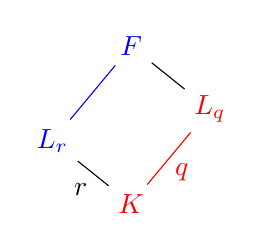
\begin{tikzpicture}

            \node [red] (Q1) at (0,0) {$K$};
            \node [red] (Q2) at (1,1.2) {$L_q$};
            \node [blue] (Q3) at (0,2) {$F$};
            \node [blue] (Q4) at (-1,0.8) {$L_r$};
        
            \draw [red] (Q1)--(Q2) node [pos=0.8, below,inner sep=0.25cm] {$q$};
            \draw (Q1)--(Q4) node [pos=0.9, below,inner sep=0.25cm] {$r$};
            \draw [blue] (Q3)--(Q4);
            \draw (Q2)--(Q3);
        
        \end{tikzpicture}
        \caption[short]{Subfields of a $C_{pq}$-extension}
    \end{figure}

    Again, the result follows immediately from the table and \eqref{eqn_local_contr}.
    
\end{proof}

We are finally ready to prove the main result of this section, from which Theorem \ref{thm_consistent_cyclic} will follow. 

\begin{lemma}\label{lem_Cd_odd}
    Let $d$ be a composite, odd squarefree integer and let $F/K$ be a Galois extension of number fields such that $\Gal(F/K)=C_{d}$. Let $E/\QQ$ be an elliptic curve and let $L_k$ be the fields as above. Then
    $$\prod_{k\mid d}(C_{E/L_k})^{\mu(d/k)}$$
    is always a rational square.
\end{lemma}

\begin{proof}
    Let $n$ be the number of distinct prime numbers dividing $d$, so that $d=p_1\ldots p_n$ for some distinct odd primes $p_i$. We prove this result by induction. The base case for $n=2$ is the content of Lemma \ref{lem_Cpq}. Assume that the result holds for squarefree cyclic Galois extensions with $n-1$ prime factors and consider the two sets of fields
    $$\mathcal{A}=\{L_k:p_n\nmid k\}\quad\text{and}\quad\mathcal{B}=\{L_k:p_n\mid k\},$$
    which are clearly a partition of all intermediate fields of $F/K$. Furthermore, the fields in $\mathcal{A}$ are precisely the intermediate fields of $L_{d/p_n}/K$, while the fields in $\mathcal{B}$ are the intermediate fields of $F/L_{p_n}$. However, since $\Gal(L_{d/p_n}/K)=\Gal(F/L_{p_n})=C_{d/p_n}$, it follows from the inductive hypothesis applied to $L_{d/p_n}/K$ and $F/L_{p_n}$ respectively that
    $$\prod_{k\mid \frac{d}{p_n}}(C_{E/L_k})^{\mu\left(\frac{d}{kp_n}\right)}\quad\text{and}\quad\prod_{p_n\mid k\mid d}(C_{E/L_{k}})^{\mu\left(d/k\right)}$$
    are both rational squares. By the natural decomposition
    $$\prod_{k\mid d}(C_{E/L_k})^{\mu(d/K)}=\prod_{k\mid \frac{d}{p_n}}(C_{E/L_k})^{\mu\left(d/k\right)}\prod_{p_n\mid k\mid d}(C_{E/L_{k}})^{\mu\left(d/k\right)}=\left(\prod_{k\mid \frac{d}{p_n}}(C_{E/L_k})^{\mu\left(\frac{d}{kp_n}\right)}\right)^{-1}\prod_{p_n\mid k\mid d}(C_{E/L_{k}})^{\mu\left(d/k\right)},$$
    it follows that the left hand side is also a rational square, as desired.
    \begin{figure}[!ht]
        \centering
        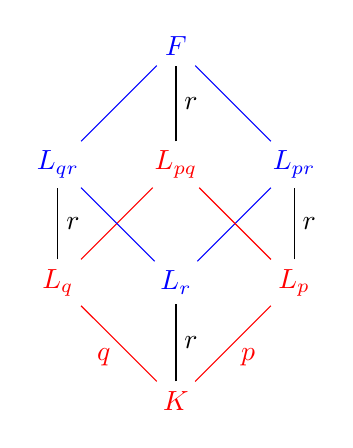
\begin{tikzpicture}

            \node [red] (Q1) at (0,0) {$K$};
            \node [red] (Q2) at (-1.5,1.5) {$L_q$};
            \node [blue] (Q3) at (0,1.5) {$L_r$};
            \node [red] (Q4) at (1.5,1.5) {$L_p$};
            \node [blue] (Q5) at (-1.5,3) {$L_{qr}$};
            \node [red] (Q6) at (0,3) {$L_{pq}$};
            \node [blue] (Q7) at (1.5,3) {$L_{pr}$};
            \node [blue] (Q8) at (0,4.5) {$F$};

            \draw [red] (Q1)--(Q2) node [pos=0.7, below,inner sep=0.25cm] {$q$};
            \draw [red] (Q1)--(Q4) node [pos=0.7, below,inner sep=0.25cm] {$p$};
            \draw (Q1)--(Q3) node [pos=0.5, right,inner sep=0.1cm] {$r$};
            \draw (Q2)--(Q5) node [pos=0.5, right,inner sep=0.1cm] {$r$};
            \draw (Q2)--(Q6) [red];
            \draw (Q3)--(Q5) [blue];
            \draw (Q3)--(Q7) [blue];
            \draw (Q4)--(Q6) [red];
            \draw (Q4)--(Q7) node [pos=0.5, right,inner sep=0.1cm] {$r$};
            \draw (Q5)--(Q8) [blue];
            \draw (Q6)--(Q8) node [pos=0.5, right,inner sep=0.1cm] {$r$};
            \draw (Q7)--(Q8) [blue];
        
        \end{tikzpicture}
        \caption[short]{Partition of $n=3$ into $n=2$. Red fields are in $\mathcal{A}$ while blue fields are in $\mathcal{B}$.}
    \end{figure}
\end{proof}

The proof of Theorem \ref{thm_consistent_cyclic} for odd $d$ is now straightforward.

\begin{proof}[Theorem \ref{thm_consistent_cyclic} for odd $d$]
    The proof is divided into two cases depending on whether $d$ is the power of a prime or not. Suppose first that $d$ is not, so that $\rad(d)$ is a squarefree \textbf{composite} number. However, by Remark \ref{rem_radical} and Lemma \ref{lem_Cd_odd} we know that 
    $$\frac{\prod_i C_{E/F_i}}{\prod_j C_{E/F'_j}}$$
    is a rational square, and therefore it is the norm of an element for any quadratic extension of $\QQ$. 

    If $d=q^n$ for some odd prime $q$ and $n\geq1$, then Lemma \ref{lem_cyclic_decomp} and Lemma \ref{lem_Cp} show that 
    $$\frac{\prod_i C_{E/F_i}}{\prod_j C_{E/F'_j}}=\frac{C_{E/F}}{C_{E/L_{p^{n-1}}}}$$ is a norm from $\QQ(\sqrt{q^*})$, and by Lemma \ref{lem_subfields} this is the only quadratic subfield of $\QQ(\zeta_{q^n})$ so the result follows.
\end{proof}
 
\subsection*{Even Cyclic Extensions}
A bit more care is required to prove Theorem \ref{thm_consistent_cyclic} for even $d$. This difficulty mainly lies in the case when $d$ is only divisible by one odd prime $p$. Likewise to the earlier case, we first prove some relevant results.

\begin{lemma}\label{lem_C2p}
    Let $q$ be an odd prime and let $F/K$ be a Galois extension of number fields such that $\Gal(F/K)=C_{2q}$ and let $L_k$ be the fields as above. Let $E/\QQ$ be an elliptic curve. Then
    $$\frac{C_{E/F}C_{E/K}}{C_{E/L_2}C_{E/L_q}}$$
    is a norm from $\QQ(\sqrt{q^*})$.
\end{lemma}

\begin{proof}
    Similarly to the proofs of Lemma \ref{lem_Cp} and \ref{lem_Cpq}, let $\pp$ be a prime in $K$. The splitting behaviour of a prime $\pp$ in $K$ is again determined by $e_\pp$ and $f_\pp$ and therefore if $\pp$ has multiplicative reduction, the following table records its contribution.

    \begin{table}[!ht]
        \centering
        \begin{tabular}{|l|l|l|l|l|l|l|}
        \hline
        $e_\pp$ & $f_\pp$  & $T_{\fP\mid \pp}(E/\QQ)$ & $T_{\fP\mid \pp}(E/L_q)$ & $T_{\fP\mid \pp}(E/L_2)$ & $T_{\fP\mid \pp}(E/F)$ & $\contr_\chi(\pp)$ \\ \hline
        $1$ & $1$ & $n;\tilde{n}$ & $n^q;\tilde{n}^q$ & $n^2;\tilde{n}^2$ & $n^{2q};\tilde{n}^{2q}$ & $\square$ \\ \hline
        $1$ & $q$ & $n;\tilde{n}$ & $n;\tilde{n}$ & $n^2;\tilde{n}^2$ & $n^2;\tilde{n}^2$ & $\square$ \\ \hline
        $1$ & $2$ & $n;\tilde{n}$ & $n^q;\tilde{n}^q$ & $n;n$ & $n^q;n^q$ & $\square$ \\ \hline
        $1$ & $2q$ & $n;\tilde{n}$ & $n;\tilde{n}$ & $n;n$ & $n;n$ & $\square$ \\ \hline
        $q$ & $1$ & $n;\tilde{n}$ & $qn;\tilde{n}$ & $n^2;\tilde{n}^2$ & $q^2n^2;\tilde{n}^2$ & $q\square;\square$ \\ \hline
        $q$ & $2$ & $n;\tilde{n}$ & $qn;\tilde{n}$ & $n;n$ & $qn;n$ & $\square$ \\ \hline
        $2$ & $1$ & $n;\tilde{n}$ & $n^q;\tilde{n}^q$ & $2n;1$ & $2^qn^q;1^q$ & $\square$ \\ \hline
        $2$ & $q$ & $n;\tilde{n}$ & $n;\tilde{n}$ & $2n;1$ & $2n;1$ & $\square$ \\ \hline
        $2q$ & $1$ & $n;\tilde{n}$ & $qn;\tilde{n}$ & $2n;1$ & $2qn;1$ & $\square$ \\ \hline
        \end{tabular}
    \end{table}

    Since $q$ is a norm from $\QQ(\sqrt{q^*})$, then $\contr_\chi(\pp)$ is also a norm. Now assume that $\pp$ has addtiive reduction and let $p\ZZ=\pp\cap\QQ$. We first consider the contribution of the Tamagawa numbers. Note that $L_q/K$ and $F/L_2$ are $C_q$ extensions and therefore their contribution is a square if $q\neq 3$ and a square up to factors of $3$ if $q=3$. In either case, this is a norm from $\QQ(\sqrt{q^*})$.

    Finally, we consider the contribution of the $D_{\fP\mid\fp}$ terms. By reescaling $\Delta_E$, the contribution does not change up to squares, so we assume that $\Delta_E=\Delta_{E,\pp}^{\min}$ and let $x=\nu_\pp(\Delta_{E,\pp}^{\min})$. Under this assumption, all terms cancel unless $\pp$ ramifies in $F$. If $e_\pp=2$, then 
    \begin{equation}\label{eqn_ep=2}
        D_{\fP\mid\fp}(E/K)=D_{\fP\mid\fp}(E/L_q)=1,\quad D_{\fP\mid\fp}(E/L_2)=N(\pp)^{\floor{\frac{2x}{12}}}\quad\text{and}\quad D_{\fP\mid\fp}(E/F)=N(\pp)^{q\floor{\frac{2x}{12}}},
    \end{equation}
    and therefore the total contribution is $N(\pp)^{(r-1)\floor{x/6}}$, a rational square. If $q\mid e_\pp$, then $q\mid N(\pp)-1$ by Proposition \ref{prop_totally_ramified}. The reasoning is now identical to Lemma \ref{lem_Cp}. Writing $N(\pp)=p^s,\ s\geq1$ and note that the contribution is a square if $s$ is even and a square up to multiples of $p$ if $s$ is odd. However, in the latter case, $p=q$ if $(L_q)_\fP/K_\pp$ is wildly ramified and $p$ splits in $\QQ(q^*)$ if $(L_q)_\fP/K_\pp$ is tamely ramified. In either case, $p$ is a norm from $\QQ(\sqrt{q^*})$.   

    The result follows again from \eqref{eqn_local_contr}.

\end{proof}

However, as soon as $d$ is divisible by $4$, the product of local factors is a rational square even if the individual contributions might not be, as the next lemma suggests. 

\begin{lemma}\label{lem_C4p}
    Let $q$ be an odd prime and let $F/K$ be a Galois extension of number fields such that $\Gal(F/K)=C_{4q}$ and let $L_k$ be the fields as above. Let $E/\QQ$ be an elliptic curve. Then
    $$\frac{C_{E/F}C_{E/L_2}}{C_{E/L_4}C_{E/L_{2q}}}$$
    is a norm from $\QQ(i),\QQ(\sqrt{q})$ and $\QQ(\sqrt{-q})$. Moreover, if $\pp$ is a prime in $K$, then $\contr_\chi(\pp)$ is a rational square unless $E$ has additive reduction at $\pp$ and $\pp$ is totally ramified in $F/K$.
\end{lemma}

\begin{proof}
    All fields appearing in the product are intermediate fields of $L_2$ and $F$, and $\Gal(F/L_2)=C_{2q}$. Let $\pp$ be a prime in $K$, let $\bar\pp\mid\pp$ be a prime above $\pp$ in $L_2$ and let $p\ZZ=\pp\cap\QQ$.. Lemma \ref{lem_C2p} shows that if $E$ has multiplicative reduction over $\bar\pp$, $\contr_\chi(\bar\pp)$ is a square unless $e_{\bar\pp}=q$ and $f_{\bar\pp}=1$ oveer $F$. That is, $\bar\pp$ ramifies in $L_{2q}/L_2$ and is split in $L_4/L_2$, and this forces $\pp$ to split in $L_2/K$ too. Hence, $\pp=\bar\pp\bar\pp'$ for two \textbf{distinct} primes in $K$ that have the same splitting behaviour and therefore $\contr_\chi(\pp)=\contr_\chi(\bar\pp)\contr_\chi(\bar\pp')=\contr_\chi(\bar\pp)^2$ is a rational square, as desired.

    \begin{figure}[!ht]
        \centering
        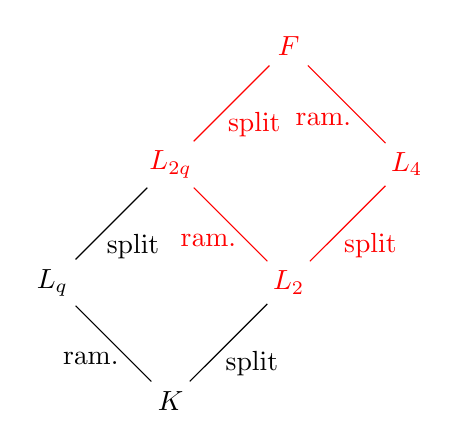
\begin{tikzpicture}

            \node (Q1) at (0,0) {$K$};
            \node (Q2) at (-1.5,1.5) {$L_q$};
            \node [red] (Q3) at (3,3) {$L_4$};
            \node [red] (Q4) at (1.5,1.5) {$L_2$};
            \node [red] (Q5) at (1.5,4.5) {$F$};
            \node [red] (Q6) at (0,3) {$L_{2q}$};
            

            \draw (Q1)--(Q2) node [pos=0.8, below,inner sep=0.4cm] {ram.};
            \draw (Q1)--(Q4) node [pos=0.8, below,inner sep=0.4cm] {split};
            \draw (Q2)--(Q6) node [pos=0.8, below,inner sep=0.4cm] {split};
            \draw [red] (Q3)--(Q5) node [pos=0.8, below,inner sep=0.4cm] {ram.};
            \draw [red] (Q4)--(Q6) node [pos=0.8, below,inner sep=0.4cm] {ram.};
            \draw [red] (Q6)--(Q5) node [pos=0.8, below,inner sep=0.4cm] {split};
            \draw [red] (Q4)--(Q3) node [pos=0.8, below,inner sep=0.4cm] {split};
        \end{tikzpicture}
        \caption[short]{\centering Field diagram for a $C_{4q}$ extension, together with the splitting\\ behaviour of a prime $\pp$ in $L_2$ with $e_\pp=q$ and $f_\pp=1$ over $F$.}
    \end{figure}

    Assume now that $E$ has additive reduction over $\bar\pp$. When $q=3$, controlling the Tamagawa numbers is lengthy, so we leave it for the end. We consider first the contribution from the $D_{\fP\mid\fp}$ terms, which is trivial unless $\bar\pp$ ramifies in $L/F_2$ (equivalently, $\pp$ ramifies in $L/K$). If $\pp$ is inert in $L_2/K$, then $N(\bar{\pp})$ is square and hence the size of all residues fields above $\pp$ are also squares. By Lemma \ref{lem_Dterms}, we get squared contribution. If $\pp=\bar\pp\bar\pp'$ splits, then $D_{\fP\mid\bar\fp}(E/L_k)=D_{\fP\mid\bar\fp'}(E/L_k)$ for every $k$, and therefore the contribution from $\pp$ is a square too. Hence, $\pp=\bar\pp^2$ ramifies in $L_2/K$, which implies that $\bar\fp$ also ramifies in $L_4/L_2$. On the other hand, if $\bar\pp$ is unramified at $L_{2q}/L_2$, \eqref{eqn_ep=2} during the proof of Lemma \ref{lem_C2p} shows that the contribution is also a square. 

    We are therefore left with the case where $\pp$ is totally ramified in $F/K$, and Propostion \ref{prop_totally_ramified} implies that $4q\mid N(\pp)-1$. Assuming again that $\Delta_E=\Delta_{E,\pp}^{\min}$ and letting $x=\nu_{\pp}(\Delta_{E,\pp}^{\min})$, Lemma \ref{lem_Dterms} imples that the $D_{\fP\mid\fp}$ terms contribute a total of 
    $$N(\pp)^{\floor{\frac{x}{6}}-\floor{\frac{x}{3}}-\floor{\frac{qx}{6}}+\floor{\frac{qx}{3}}}.$$
    Again, the parity of the expression only depends on $q,x\pmod{12}$. One can easily check that for $x\in\{2,3,4,6,8,9,10\}$, the above expression is a square unless $q\equiv 3\pmod{4}$. Write $N(\pp)=p^s$, which satisfies $p^s\equiv1\pmod{4q}$. If $s$ is even, then the contribution is clearly a square, so assume that $s$ is odd. Since $p^s\equiv1\pmod{4}$, this implies that $p\equiv1\pmod{4}$ and hence $p$ is a norm from $\QQ(i)$, which implies that $\contr_\chi(\pp)$ is a norm from $\QQ(i)$ too. Furthermore, the fact that $p^s\equiv1\pmod{4q}$ implies that
    $$\left(\frac{-q}{p}\right)=\left(\frac{q}{p}\right)=\left(\frac{p}{q}\right)=\left(\frac{p^s}{q}\right)=1,$$
    and therefore $p$ splits both in $\QQ(\sqrt{q})$ and $\QQ(\sqrt{-q})$. Since both fields have odd class number (Theorem \ref{thm_class_number}), it follows that $p$, and therefore $N(\pp)$ are norms from $\QQ(\sqrt{q})$ and $\QQ(\sqrt{-q})$ as desired. 

    Finally, we discuss Tamagawa numbers. Note that $L_{2q}/L_2$ and $F/L_4$ are $C_q$ extensions and therefore by Lemma \ref{lem_Cp} the Tamagawa numbers have a square contribution if $q\neq3$. If $q=3$, more work is required. From Lemma \ref{lem_Dterms}, we see that the Tamagawa numbers can only contribute factors of $2$ and $3$. In Lemma \ref{lem_nottwo} we showed that in $C_3$ extensions we cannot get a factor of $2$. Since $3$ is not a norm from $\QQ(\sqrt{3})$, we now need to show that we cannot get a factor of $3$ either. 
    %Upon inspection of Lemma \ref{lem_Dterms}, this only happens if $F_\fP/K_\fp$ is ramified, $\gcd(n,4)=12$ and $\sqrt{B}\in F$.
    
    We also prove this result as a separate lemma, from which the result follows.

    %{\color{red} We need to ensure that $3$ cannot appear as a factor, as otherwise we would have rank growth! That's because $3$ is not a norm of $\QQ(\sqrt{3})\subseteq\QQ(\zeta_{12})$.}
    
\end{proof}

\begin{lemma}
    Let $L/K$ be a Galois extension of number fields with $\Gal(L/K)=C_{12}$ and let $L_k$ be the intermediate fields with $[L_k:K]=k$. Let $E/\QQ$ be an elliptic curve and let $\pp$ be a prime in $K$ such that $E$ has potentially good reduction at $\pp$. If $\chi$ is a faithful character of $C_{12}$, then $$T_\chi(\pp):=\frac{T_{\fP\mid\fp}(E/F)T_{\fP\mid\fp}(E/L_2)}{T_{\fP\mid\fp}(E/L_6)T_{\fP\mid\fp}(E/L_4)}$$ is a rational square.
\end{lemma}
\begin{proof}
    Let $\bar\pp$ be a prime in $L_2$ above $\pp$ and let $n=\nu_{\bar\pp}(\Delta_{E,\bar\pp}^{\min})$ be the minimal disciminant of $E$ at $\bar\pp$. The proof is divided in three cases, depending on the splitting behaviour of $\pp$ in $L_2$. If $\pp$ splits in $L_2/K$, then $\pp=\bar\pp\bar\pp'$ with $T_\chi(\bar\pp)=T_\chi(\bar\pp')$. Therefore, $T_\chi(\pp)=T_\chi(\bar\pp)T_\chi(\bar\pp')$ is a square. Next, suppose that $\pp$ is inert in $L_2/K$. This implies that $\bar\pp$ is also inert in $L_4/L_2$ and if $\fP$ is the prime in $L_4$ above $\bar\pp$, then the valuation of the minimal discriminant of $E$ at $\fP$ is also $n$. Since the splitting behaviour of $\bar\pp$ in $L_6/L_2$ coincides with the splitting behaviour of $\fP$ in $F/L_4$, then 
    $$\frac{T_{\fP\mid\fp}(E/F)}{T_{\fP\mid\fp}(E/L_4)}=\frac{T_{\fP\mid\fp}(E/L_6)}{T_{\fP\mid\fp}(E/L_2)},$$
    and therefore $T_\chi(\pp)=1$.

    Finally, assume that $\pp$ ramifies in $L_2/K$ so that $\pp=\bar\pp^2$. This immediately implies that $\bar\pp$ also ramifies in $L_4/L_2$. From Lemma \ref{lem_Cp}, we also know that in $C_3$ extensions the Tamagawa numbers above some prime contribute a square unless the prime ramifies. Hence, we may also assume that $\pp$ ramifies in $L_3/K$ and therefore $\pp$ is totally ramified in $F/K$. Using Lemma \ref{lem_add_tam}, one can easily show that the Tamagawa numbers cancel out if $\gcd(n,12)\in\{3,4,6,12\}$, so we only need to consider the case $\gcd(n,12)=2$. However, recall that $E$ has potentially good reduction at $\pp$, and since $\pp=\bar\pp^2$ ramifies, then the valuation of the minimal discrimiant at $\pp$ is $n/2$ or $(n+12)/2$. But then $\gcd(\nu_\pp(\Delta_{E,\pp}^{\min}),12)=\gcd(n/2,12)=1$, a contradiction.
\end{proof}


We are now ready to prove Theorem \ref{thm_consistent_cyclic} for even $d$. We break down the proof into three cases:

\subsubsection*{Case 1: $d$ is not divisible by any odd prime, so $d=2^l$}
If $l=1$, then $\QQ(\zeta_2)=\QQ$, so there is nothing to prove, so assume that $l\geq2$. If $\Gal(F/\QQ)=C_{2^l}$, then 
$$\frac{\prod_i C_{E/F_i}}{\prod_j C_{E/F'_j}}=\frac{C_{E/F}}{C_{E/L_{2^{l-1}}}},$$
and by Lemma \ref{lem_Cp}, we know that this is a rational square up to factors of $2$, so it suffices to show that $2$ is a norm of every quadratic subfield of $\QQ(\zeta_{2^l})$. A standard argument shows that $\Gal(\QQ(\zeta_{2^l})/\QQ)=(\ZZ/2^l\ZZ)^*=C_{2^{l-2}}\times C_2$ and therefore $\QQ(\zeta_{2^l})$ has $\QQ(i)$ as its unique quadratic subextension if $l=2$ and has three quadratic subextensions if $l\geq 3$. Note that $\zeta_8=(1+i)/\sqrt{2}$ and therefore $\QQ(\zeta_8)=\QQ(i,\sqrt{2})$. The three quadratic subextensions are therefore $\QQ(i), \QQ(\sqrt{2})$ and $\QQ(\sqrt{-2})$. Then the result follows from the fact that 
$$2=\Norm_{\QQ(i)}(1+i)=\Norm_{\QQ(\sqrt{-2})}(2)=\Norm_{\QQ(\sqrt{2})}(2+\sqrt{2}).$$

\subsubsection*{Case 1: $d$ is divisible by at least two odd primes}
Let $K=L_{d/\rad(d)}$ be as in Remark \ref{rem_radical} such that $\Gal(F/K)=C_{\rad(d)}$ and all fields appearing in the product of local factors contain $K$. Then using the same idea as in Lemma \ref{lem_Cd_odd}, let 
$$\mathcal{A}=\{L_k\supseteq K:2\nmid [L_k:K]\}\quad\text{and}\quad\mathcal{B}=\{L_k\supseteq K:2\mid [L_k:K]\}.$$
Then the fields in $\mathcal{A}$ and $\mathcal{B}$ are the intermediate fields of (distinct!) $C_{\rad(d)/2}$ extensions. These are odd cyclic extensions, and therefore by Lemma \ref{lem_Cd_odd} the contribution is a rational square and therefore a norm from any quadratic extension.

\subsubsection*{Case 3: $d$ is divisible by one odd prime}
In this case, write $d=2^lp^n$ and let $L_k$ be the fields as above. In this case, we note that 
$$\frac{\prod_i C_{E/F_i}}{\prod_j C_{E/F'_j}}=\frac{C_{E/F}C_{E/L_{d/2p}}}{C_{E/L_{d/2}}C_{E/L_{d/p}}}.$$
By Lemma \ref{lem_Cp}, we know that this product is a square up to multiples of $p$. If $l=1$, then $\Gal(\QQ(\zeta_{2p^n})/\QQ)=(\ZZ/2p^n\ZZ)^*=(\ZZ/p^n\ZZ)^*$ is cyclic, and therefore the unique quadratic subfield is $\QQ(\sqrt{p^*})$, and we already know that $p$ is a norm of this field.

From Lemma \ref{lem_C2p} that the contribution of $p$ comes from those primes $\pp$ in $L_{d/2p}$ such that they ramify in $L_{d/2}$ and they split in $L_{d/p}$. However, as in the proof of Lemma \ref{lem_C4p}, the prime $\bar{\pp}=\pp\cap L_{d/4p}$ must also split in $L_{d/2p}$ so $\bar{\pp}=\pp\pp'$ for $\pp'\neq\pp$ in $L_{d/2p}$. Since $\pp$ and $\pp'$ have the same splitting behaviour, they give the same contribution. Hence, the product of local terms is in fact a rational square and therefore the norm of any quadratic extension.

This concludes the proof of Theorem \ref{thm_consistent_cyclic}, and we have in addition shown that the contribution is always a square except when $d=2^n,p^n$ or $2p^n$, where $p$ is an odd rational prime.
\qed




\subsection{Odd-Degree Extensions}